\documentclass{beamer}
\mode<presentation>
\usetheme{CambridgeUS}
\usepackage[russian]{babel}
\usepackage[utf8]{inputenc}
\usepackage[T2A]{fontenc}
\usepackage{sansmathaccent}

\usepackage{verbatim}
\usepackage{alltt}

\pdfmapfile{+sansmathaccent.map}
\title[Подпрограммы]{Функции и процедуры}
\author{Наумов Д.А., доц. каф. КТ, ИТГД }
\date[01.04.2019] {Алгоритмические языки и программирование, 2019}

\begin{document}

%ТИТУЛЬНЫЙ СЛАЙД
\begin{frame}
  \titlepage
\end{frame}
  
%СОДЕРЖАНИЕ ЛЕКЦИИ
\begin{frame}
  \frametitle{Содержание лекции}
  \tableofcontents  
\end{frame}
  
%РАЗДЕЛ 1
\section{Подпрограммы: процедуры и функции}
\subsection{Подпрограммы}
\begin{frame}
\begin{block}{Подпрограмма}
идентифицированная часть компьютерной программы, содержащая описание определённого набора действий, которая может быть многократно вызвана из разных частей программы.
\end{block}
Назначение подпрограмм:
\begin{itemize}
\item выделить целостную подзадачу, имеющую типовое решение;
\item сделать программу более понятной и обозримой.
\end{itemize}
Преимущества подпрограмм:
\begin{enumerate}
\item декомпозиция сложной задачи;
\item уменьшение дублирования кода;
\item возможность повторного использования кода;
\item разделение задач между исполнителями или стадиями проекта;
\item сокрытие деталей реализации;
\item упрощение отладки.
\end{enumerate}
\end{frame} 

\subsection{Описание функций}
\begin{frame}[fragile]
Виды подпрограмм в языке \textit{Pascal}: \textbf{функции} и \textbf{процедуры}. Синтаксическая форма описания функции:
\begin{alltt}
1 function <ИмяФункции>([<СписокФормПарам>]):<ТипВозврЗнач>;
2     [<РазделОписаний>]
3 begin
4   <Оператор1>;
5   <Оператор2>;
6   ...;
7   <Оператор3>;
8 end;
\end{alltt}
\begin{itemize}
\item $<$ ИмяФункции $>$ - имя функции, идентификатор;
\item $<$ СписокФормПарам $>$ - список формальных параметров с указанием их типа.
\item $<$ ТипВозврЗнач $>$ - тип значения, возвращаемого функцией.
\item $<$ РазделОписаний $>$ - раздел описаний локальных меток, констант, переменных, типов данных, процедур и функций.
\end{itemize}
\end{frame}

\begin{frame}[fragile]
Пример описания функции для вычисления степени с натуральным показателем:
\begin{alltt}
1 function CalcPower(x: real; n: integer):real;
2 var 
3   i: integer;
4   p: real;
5 begin
6   p := 1;
7   for i := 1 to n do 
8       p := p * x;
9   CalcPower := p; (*возвращаем значение*)
10 end;
\end{alltt}
\begin{itemize}
\item x, n - формальные параметры;
\item i, p - локальные переменные;
\end{itemize}
\end{frame}

\begin{frame}[fragile]
При обращении к функции происходит:
\begin{enumerate}
\item вычисление значений фактических параметров (слева направо);
\item подстановка значений фактических параметров на место формальных параметров;
\item выполнение операторов тела функции;
\item возврат значения функции в основную программу;
\item возврат управления в точку вызова;
\end{enumerate}
Вычисление выражения $z = x^{5} + (x+1)^{3}$:
\begin{alltt}
11 var x, z: real; 
12 begin
13   x := 1.001;
14   z := CalcPower(x, 5) + CalcPower(x+1, 3);
15   writeln('x=', x:6:4, 'z=', z:6:4);
16 end.
\end{alltt}
\end{frame}

\begin{frame}[fragile]
\begin{itemize}
\item вызов функции должен осуществляться в некотором выражении (иначе "потеряется" возвращаемое значение);
\end{itemize}
\begin{alltt}
1 function Tan(x: real):real;
2 begin
3   Tan := Sin(x)/Cos(x);
4 end;
5 begin
6   Tan(Pi/4); //возвращаемое значение "теряется"
7 end.
\end{alltt}
\end{frame}

\begin{frame}[fragile]
\begin{itemize}
\item в теле функции должен выполниться хотя бы раз оператор вида \textit{ИмяФункции := Значение} (иначе возвращаемое значение будет неопределено).
\end{itemize}
\begin{alltt}
1 function IsLeapYear(aYear: integer):boolean;
2 begin
3   if aYear div 400 = 0 then
4      IsLeapYear := true
5   else if aYear div 100 = 0 then
6      IsLeapYear := false
7   else if aYear div 4 = 0 then
8      IsLeapYear := true;
9 end;
\end{alltt}
\end{frame}

\subsection{Описание процедуры}
\begin{frame}[fragile]{Синтаксическая форма описания процедуры}
\begin{alltt}
1 procedure <ИмяПроцедуры>([<СписокФормПарам>]);
2     [<РазделОписаний>]
3 begin
4   <Оператор1>;
5   <Оператор2>;
6   ...;
7   <Оператор3>;
8 end;
\end{alltt}
\begin{itemize}
\item $<$ ИмяПроцедуры $>$ - имя функции, идентификатор;
\item $<$ СписокФормПарам $>$ - список формальных параметров с указанием их типа.
\item $<$ РазделОписаний $>$ - раздел описаний локальных меток, констант, переменных, типов данных, процедур и функций.
\end{itemize}
\end{frame}

\begin{frame}{Блочный принцип организации программы}
Программа, процедура или ункция представляют собой блоки со своими разделами описаний и определений, которые могут быть вложены друг в друга. 
\begin{block}{Внешний блок}
блок, содержащий в своем описании другие блоки (по отношению к этим блокам).
\end{block}
Объекты, описанные во внешнем блоке, и не имеющие других описаний, являются глобальными для внутренних блоков.
\begin{block}{Внутренний блок}
блок, содержащийся в другом блоке.
\end{block}
Объекты, описанные внутри блока, являются локальными по отношению к нему, не доступны во внешних блоках, но доступны во внутренних блоках начиная с момента описания. 
\end{frame}

\begin{frame}
\begin{block}{Области видимости}
\begin{center}
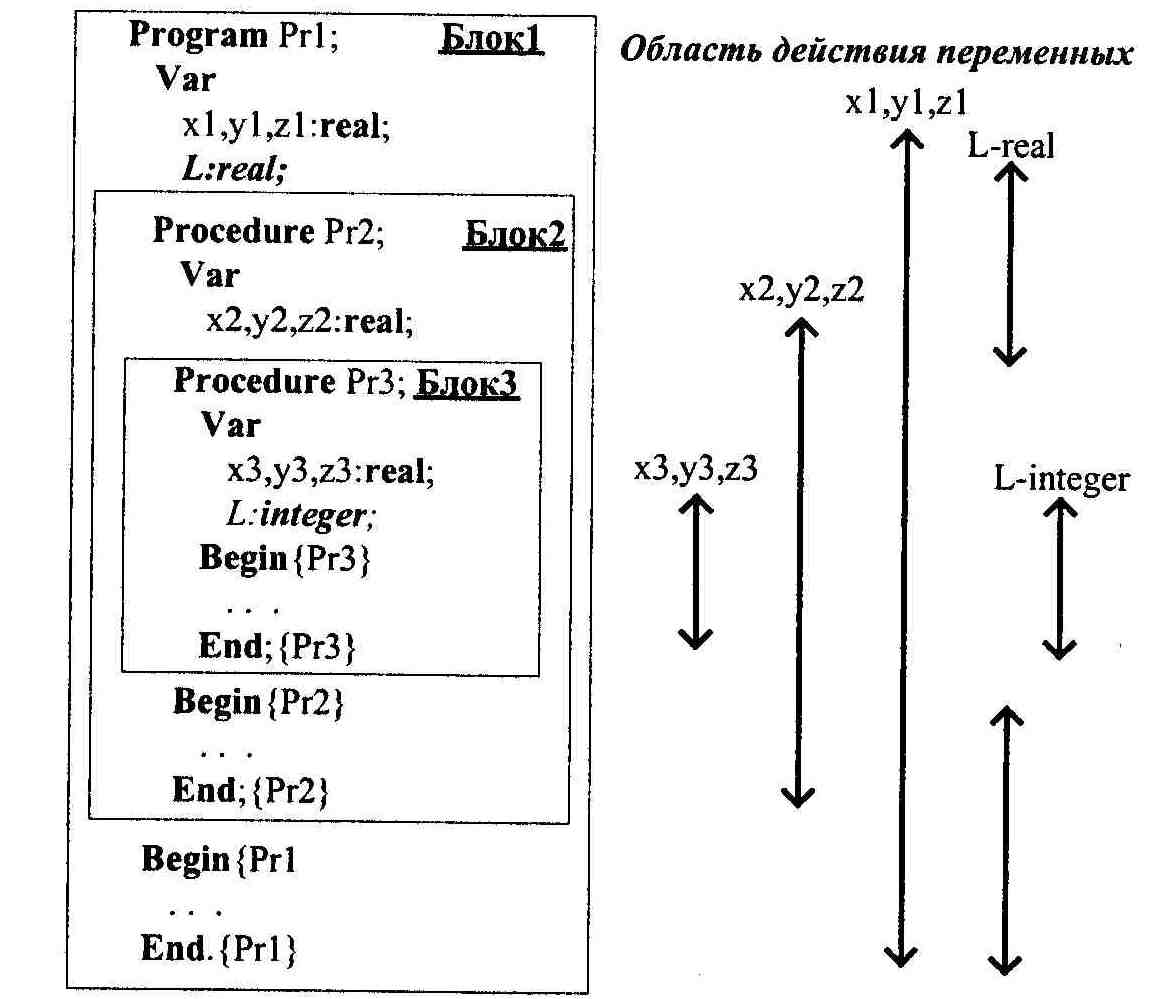
\includegraphics[scale=0.8]{images/block.jpg}
\end{center}
\end{block}
\end{frame}

\begin{frame}[fragile]{Обмен данным с подпрограммой}
\begin{itemize}
\item обмен данными между подпрограммами осуществляется при помощи формальных и фактических параметров.
\item использование глобальных переменных для обмена данных не рекомендуется, так как это усложняет разработку и отладку, и может привести к неконтролируемому изменению данных и контекста выполнения;
\item для передачи нестандратных типов данных необходимо их описание в разделе \textbf{type}.
\end{itemize}
\begin{alltt}
1 type
2   TComplex = record
3     Re, //вещественная часть
4     Im: TСElem; //мнимая часть
5   end;
6 procedure Add(const A, B: TComplex; var C: TComplex); 
\end{alltt}
\end{frame}

\begin{frame}[fragile]
Процедура сортировки массива:
\begin{alltt}
1 type
2   TIndex = 1..10;
3   TElem = real;
4   TArray = array[TIndex] of TElem;
5 procedure Sort(var V:TArray; const n:TIndex); 
6 var
7   i, j: TIndex;
8   tmp:  TElem;
9 begin
10  for i := 1 to n-1 do
11    for j := i + 1 to n do
12      if V[i] > V[j] then
13      begin
14        tmp := V[i]; V[i] := V[j]; V[j] := tmp;
15      end;
16 end;
\end{alltt}
\end{frame}

\begin{frame}[fragile]
При обращении к процедуре происходит:
\begin{itemize}
\item вычисление значений фактических параметров (слева направо);
\item подстановка значений фактических параметров на место формальных параметров;
\item выполнение операторов тела процедуры;
\item возврат управления в точку вызова;
\end{itemize}
Сортировка массива:
\begin{alltt}
11 var vector: TVector; 
12 var i: TIndex; 
13 begin
14   for i := 1 to 10 do
15      vector[i] := random(100);
16   Sort(vector, 10);
17 end.
\end{alltt}
Вызов процедуры должен осуществляться в отдельном операторе.
\end{frame}

\begin{frame}[fragile]{Виды формальных параметров подпрограмм}
\begin{itemize}
\item параметры-значения;
\item параметры-переменные;
\item параметры-константы;
\item параметры процедурного (функционального) типа.
\end{itemize}
\begin{alltt}
1 type
2   TArray = array[1..100] of real;
3   TFunction = function(x: real):real; 
4  //x - параметр-значение
5 function Sqr(x: real): real;
6  //v - параметр-переменная
7 procedure Sort(var v: TArray; n: integer);
8  //m - параметр-константа
9 function Find(x: real; const m: TArray; n: integer): real;
10 //f - параметр функционального типа
11 function Integral(a, b: real; f: TFunction): real;
\end{alltt}
\end{frame}

\begin{frame}[fragile]{Параметры-значения}
\begin{block}{Параметры-значения }
формальные параметры, описанные в загловоке подпрограммы без использования ключевых слов var или const, и не являющиеся параметрами процедурного типа.
\end{block}
\begin{itemize}
\item для чего нужны: передача входных данных в подпрограмму;
\item как передается: по значению (в стеке создается копия значения актического параметра), которая после завершения подпрограммы уничтожается;
\item может ли изменяться внутри подпрограммы: да;
\item влияет ли изменение формального параметра на фактический: нет;
\item что может являться актическим параметром: выражение, совместимое по присваиванию с типом формального параметра.
\end{itemize}
\end{frame}

\begin{frame}[fragile]{Параметры-значения}
\begin{alltt}
1 function IsIdentifier(s: string): boolean;
2 const 
3   LETTERS = ['A'..'Z', 'a'..'z'];
4   DIGITS = ['0'..'9'];
5 begin
6   if not (s[1] in LETTERS + ['_']) then begin
7     IsIdentifier := false;
8     exit; //выход из подпрограммы
9   end else	
10   for i: integer := 2 To length(s) do
11     if not (s[i] In LETTERS + DIGITS + ['_']) then begin
12        IsIdentifier := false;
13        exit; //выход из подпрограммы
14     end;
15   IsIdentifier := true;
16 end.
\end{alltt}
\end{frame}

\begin{frame}[fragile]{Параметры-переменные}
\begin{block}{Параметры-переменные}
это формальные параметры, описанные в загловоке подпрограммы с использованием ключевого слова \textbf{var}.
\end{block}
\begin{itemize}
\item для чего нужны: передача входных данных в подпрограмму и выходных данных в программу;
\item как передается: по адресу фактического параметра;
\item может ли изменяться внутри подпрограммы: да;
\item влияет ли изменение формального параметра на фактический: да;
\item что может являться фактическим параметром: L-value ( выражение, указывающее на переменную (область памяти для хранения изменяемого значения) соответствующего типа).
\end{itemize}
Вопрос: использовать ли параметры-переменные для функции?
\end{frame}

\begin{frame}[fragile]{Параметры-переменные}
\begin{alltt}
//do: получение частного комплексных чисел
//in: A - делимое, B - делитель
//out: С - частное A / B
1 procedure Div(const A, B: TComplex; var C: TComplex; 
    var ErrorCode: integer);
2  var d: TCElem;
3  begin
4    d := B.Re * B.Re + B.Im * B.Im;
5    if abs(d) < 1e-10 then begin
7      ErrorCode := -1;
8      exit;
9    end;
10   ErrorCode := 0;
11   C.Re := (A.Re * B.Re + A.Im * B.Im) / d;
12   C.Im := (A.Im * B.Re - A.Re * B.Im) / d;
13 end;	
\end{alltt}
\end{frame}

\begin{frame}[fragile]{Параметры-константы}
\begin{block}{Параметры-константы}
формальные параметры, описанные в загловоке подпрограммы с использованием ключевого слова \textbf{const}.
\end{block}
\begin{itemize}
\item для чего нужны: передача входных данных в подпрограмму с контролем из неизменности;
\item как передается: по адресу фактического параметра;
\item может ли изменяться внутри подпрограммы: нет (попытка приведет к ошибке компиляции);
\item влияет ли изменение формального параметра на актический: нет;
\item что может являться фактическим параметром: выражение, совместимое по присваиванию формальным параметром.
\end{itemize}
\end{frame}

\begin{frame}[fragile]{Параметры-константы}
\begin{alltt}
 1 type 
 2  TIndex = 1..Nmax;
 3  TElem = real;
 4  TVector = array[TIndex] Of TElem;
 5 function SearchElement(const V:TVector; 
     const Element:TElem; StartIndex, EndIndex: TIndex):TIndex;
 6 var 
 7   i: TIndex;
 8 begin
 9 for i := StartIndex to EndIndex do
10   if abs(V[i] - Element) <= 1e-8 then begin
11     SearchElement := i;        
12     exit
13   end;	
14   SearchElement := -1;
15 end;
\end{alltt}
\end{frame}

\begin{frame}[fragile]
\begin{block}{Процедурный тип}
описывается в разделе \textbf{type} подобно описанию процедур и функций без указания их имени.
\end{block}
\begin{alltt}
 1 type 
 2  \{\$F+\}  
 3  TFunction = function(x:real):real;
 4  TProcedure = procedure(var x:real); 
\end{alltt}
Описание процедурного типа позволяет использовать в качестве фактических параметров процедуры и функции.
\begin{itemize}
\item подпрограмма-фактический параметр должна быть в области видимости (не локальная, не стандартная подпрограмма);
\item должны совпадать сигнатуры (тип и количество формальных параметров и возвращаемое значение) у фактического параметра-подпрограммы и формального параметра;
\item в старых компиляторах должна использоваться директива комплиятора far.
\end{itemize}
\end{frame}

\begin{frame}[fragile]{Пример использования параметра процедурного типа}
\begin{block}{Метод трапеций}
Метод трапеций — метод численного интегрирования функции одной переменной, заключающийся в замене на каждом элементарном отрезке подынтегральной функции на многочлен первой степени, то есть линейную функцию. 
\end{block}
\begin{block}{Схема для численного интегрирования}
\begin{center}
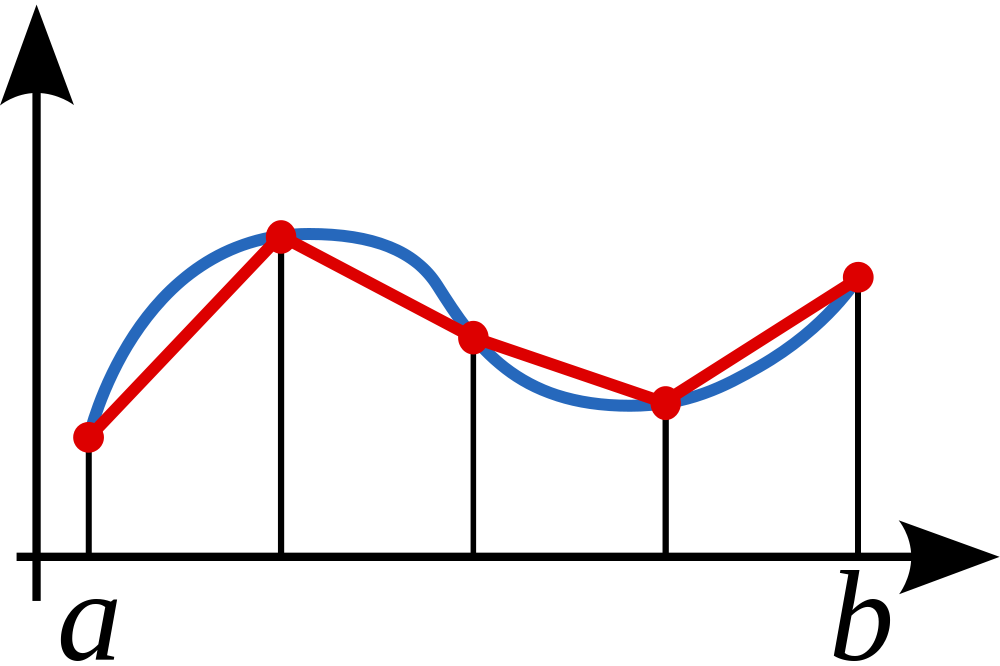
\includegraphics[scale=0.15]{images/trap.png}
\end{center}
\end{block}
\end{frame}

\begin{frame}[fragile]{Метод трапеций}
\begin{block}{Формула для интегрирования}
\begin{center}
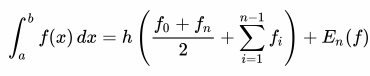
\includegraphics[scale=0.5]{images/formula.png}
\end{center}
\end{block}
\begin{alltt}
 1 type TFunction = function(x:real):real;
 2 function FSin(x: real):real;
 3 begin
 4   FSin := sin(x);
 5 end;
 6 function FCos(x: real):real;
 7 begin
 8   FCos := cos(x);
 9 end;
\end{alltt}
\end{frame}

\begin{frame}[fragile]
\begin{alltt}
//функция численного интегрирования по формуле трапеций для 
//  заданного числа шагов
1 function CalcIntegralStep(F: TFunction; LimitA, LimitB,
     Step: real): real;
2 var
3   s, x: real;  
4   i, n: integer;
4 begin
//получаем количество разбиений
5   n := round((LimitB - LimitA) / Step); 
6   s := 0;  
7   for i := 1 to n - 1 do begin
8     x := LimitA + Step * i;    
//обращаемся к параметру F функционального типа 
9     s := s + F(x); 
10  end;
11  CalcIntegralStep := Step*((F(LimitA)+F(LimitB))/2+s);
12 end;  
\end{alltt}
\end{frame}

\begin{frame}[fragile]
\begin{alltt}
//функция численного интегрирования по формуле трапеций 
//  с заданной точностью
1 function CalcIntegral(F:TFunction;LimitA,LimitB:real):real;
2 var
3  i: integer; 
4  prev, curr, step: real; 
5 begin  
6  step := (LimitB - LimitA) / FIRST_STEP;    
7  i := 0;
8  curr := CalcIntegralStep(F, LimitA, LimitB, step);
9  repeat
10   i := i + 1;       
11   step := step / 2; //уменьшаем шаг вдвое
12   prev := curr;     
13    curr := CalcIntegralStep(F, LimitA, LimitB, step);    
14  until (abs(prev - curr) < EPS) or (i > LIMIT);  
15  CalcIntegral := curr;
16 end;  
\end{alltt}
\end{frame}

\begin{frame}[fragile]{Пример сортировки массива}
\begin{alltt}
 1 //функция сравнения элементов массива
 2  TCompareFunction = function(FirstValue, 
       SecondValue: TElem):boolean;
 3 //функция сравнения элементов для сортировки по возрастанию
 4 function SortAscending(FirstValue, 
     SecondValue: TElem):boolean;
 5 begin
 6   SortAscending := FirstValue <= SecondValue;
 7 end;

 8 //функция сравнения элементов для сортировки по убыванию
 9 function SortDescending(FirstValue, 
     SecondValue: TElem):boolean;
10 begin
11  SortDescending := FirstValue >= SecondValue;
12 end;
\end{alltt}
\end{frame}

\begin{frame}[fragile]{Пример сортировки массива}
\begin{alltt}
//процедура сортировки
1 procedure Sort(var aVector: TVector; aCount: TIndex;
     aSortFunction: TCompareFunction);
2 var 
3    i, k : TIndex; tmp: TElem;
4 begin
5   for i:=1 to NMax-1 do
6     for k:=i downto 1 do
7       //если значения расположены не в требуемом порядке
8        if not aSortFunction(aVector[k], aVector[k+1]) then
9       begin
10          tmp := aVector[k];
11          aVector[k] := aVector[k + 1];
12          aVector[k + 1] := tmp;
13         end;
14 end;
\end{alltt}
\end{frame}

\begin{frame}[fragile]{Пример сортировки массива}
\begin{alltt}
//сортируем по возрастанию, передавая в качестве параметра 
//функцию SortAscending

Sort(MyVector, NMax, SortAscending);

//сортируем по убыванию, передавая в качестве параметра 
//функцию SortDescending  

Sort(MyVector, NMax, SortDescending);
\end{alltt}
\end{frame}

%РАЗДЕЛ 2
\section{Варианты заданий}
\begin{frame}{Варианты заданий}
\textbf{Вариант 1}. Дана целочисленная прямоугольная матрица. Определить:
\begin{enumerate}
\item количество строк, не содержащих ни одного нулевого элемента (оформить в виде функции);
\item максимальное из чисел, встречающихся в заданной матрице более одного раза (оформить в виде процедуры).
\end{enumerate}
\textbf{Вариант 2}. Дана целочисленная прямоугольная матрица. Определить:
\begin{enumerate}
\item количество столбцов, не содержащих ни одного нулевого элемента (оформить в виде функции); 
\item Характеристикой строки целочисленной матрицы назовем сумму ее положительных четных элементов. Переставляя строки заданной матрицы, расположить их в соответствии с ростом характеристик (оформить в виде процедуры).
\end{enumerate}
\end{frame} 

\begin{frame}{Варианты заданий}
\textbf{Вариант 3}. Дана целочисленная прямоугольная матрица. Определить:
\begin{enumerate}
\item количество столбцов, содержащих хотя бы один нулевой элемент (оформить в виде функции);
\item номер строки, в которой находится самая длинная серия одинаковых элементов (оформить в виде процедуры).
\end{enumerate}
\textbf{Вариант 4}. Дана целочисленная квадратная матрица. Определить:
\begin{enumerate}
\item произведение элементов в тех строках, которые не содержат отрицательных элементов (оформить в виде функции); 
\item максимум среди сумм элементов диагоналей, параллельных главной диагонали матрицы (оформить в виде процедуры).
\end{enumerate}
\end{frame} 

\begin{frame}{Варианты заданий}
\textbf{Вариант 5}. Дана целочисленная квадратная матрица. Определить:
\begin{enumerate}
\item сумму элементов в тех столбцах, которые не содержат отрицательных элементов (оформить в виде функции);
\item минимум среди сумм модулей элементов диагоналей, параллельных побочной диагонали матрицы (оформить в виде процедуры).
\end{enumerate}
\textbf{Вариант 6}. Дана целочисленная квадратная матрица. Определить:
\begin{enumerate}
\item такие k, что k-я строка матрицы совпадает с k-м столбцом (оформить в виде процедуры); 
\item найти сумму элементов в тех строках, которые содержат хотя бы один отрицательный элемент (оформить в виде функции).
\end{enumerate}
\end{frame}

\begin{frame}{Варианты заданий}
\textbf{Вариант 7}. Дана целочисленная квадратная матрица. Определить:
\begin{enumerate}
\item сумму элементов в тех столбцах, которые не содержат отрицательных элементов (оформить в виде функции);
\item минимум среди сумм модулей элементов диагоналей, параллельных побочной диагонали матрицы (оформить в виде процедуры).
\end{enumerate}
\textbf{Вариант 8}. Дана целочисленная прямоугольная матрица. Характеристикой столбца целочисленной матрицы назовем сумму модулей его отрицательных нечетных элементов. 
\begin{enumerate}
\item переставляя столбцы заданной матрицы, расположить их в соответствии с ростом характеристик (оформить в виде
процедуры); 
\item Найти сумму элементов в тех столбцах, которые содержат хотя бы один отрицательный элемент (оформить в виде функции).
\end{enumerate}
\end{frame}

\begin{frame}{Варианты заданий}
\textbf{Вариант 9}. Дана целочисленная квадратная матрица. Определить:
\begin{enumerate}
\item сумму элементов в тех столбцах, которые не содержат отрицательных элементов (оформить в виде функции);
\item минимум среди сумм модулей элементов диагоналей, параллельных побочной диагонали матрицы (оформить в виде процедуры).
\end{enumerate}
\textbf{Вариант 10}. 
\begin{enumerate}
\item Коэффициенты системы линейных уравнений заданы в виде прямоугольной матрицы. С помощью допустимых преобразований привести систему к треугольному виду (оформить в виде процедуры); 
\item Найти количество строк, среднее арифметическое элементов которых меньше заданной величины (оформить в виде функции).
\end{enumerate}
\end{frame}

\end{document}
